\documentclass[10pt,a4paper]{article}

\usepackage{appendix}
\usepackage{graphicx}
\usepackage{biblatex}
\usepackage{parskip}
\usepackage{listings}
\usepackage{caption}
\usepackage{subcaption}
\usepackage{amsmath}
\usepackage{listings}
\usepackage{xcolor}
\usepackage[most]{tcolorbox}

%%%%%%%%%%%%%%%%%%%%%%%%%%%%%%%%%%%%%%%%%%%%%%%%%%%%%%%%%%%%%%%%%%%%%%%%%%%%%%%%%%%%%%%%%%%%%%%%%%%%%%%%%%
\definecolor{codegreen}{rgb}{0,0.6,0}
\definecolor{codegray}{rgb}{0.5,0.5,0.5}
\definecolor{codepurple}{rgb}{0.58,0,0.82}
\definecolor{backcolour}{rgb}{1,1,1}

\lstdefinestyle{mystyle}
{
  backgroundcolor=\color{backcolour},  
  commentstyle=\color{codegreen},
  keywordstyle=\color{magenta},
  numberstyle=\tiny\color{codegray},
  stringstyle=\color{codepurple},
  basicstyle=\ttfamily\footnotesize,
  breakatwhitespace=false,     
  breaklines=true,         
  captionpos=b,          
  keepspaces=true,         
  numbers=left,          
  numbersep=5pt,         
  showspaces=false,        
  showstringspaces=false,
  showtabs=false,         
  tabsize=2
}

\lstset{style=mystyle}
%%%%%%%%%%%%%%%%%%%%%%%%%%%%%%%%%%%%%%%%%%%%%%%%%%%%%%%%%%%%%%%%%%%%%%%%%%%%%%%%%%%%%%%%%%%%%%%%%%%%%%%%%%

\lstset{basicstyle=\ttfamily, breaklines = true, tabsize=2}
\graphicspath{ {./Images/} }
\setlength{\parskip}{1em}
\begin{document}
%%%%%%%%%%%%%%%%%%%%%%%%%%%%%%%%%%%%%%%%%%%%%%%%%%%%%%%%%%%%%%%%%%%%%%%%%%%%%%%%%%%%%%%%%%%%%%%%%%%%%%%%%%

\begin{titlepage}
	\centering
	{\scshape\LARGE Imperial College London \par}
	\vspace{1cm}
    {\scshape\Large Computer Architecture: Year 2\par}
    \vspace{1.5cm}
	{\huge\bfseries 4: Performance \par}
	\vspace{2cm}
	{\Large\ Xin Wang }
	\vfill
	{\large \today\par}
\end{titlepage}

%%%%%%%%%%%%%%%%%%%%%%%%%%%%%%%%%%%%%%%%%%%%%%%%%%%%%%%%%%%%%%%%%%%%%%%%%%%%%%%%%%%%%%%%%%%%%%%%%%%%%%%%%%

\tableofcontents
\pagebreak

%%%%%%%%%%%%%%%%%%%%%%%%%%%%%%%%%%%%%%%%%%%%%%%%%%%%%%%%%%%%%%%%%%%%%%%%%%%%%%%%%%%%%%%%%%%%%%%%%%%%%%%%%%
\section{Introduction}

Assessing the performance of computers can be quite challenging. The scale and intricacy of modern
software systems have made performance assessment much more difficult.

Measuring the performance of a computer is a very relative aspect. Many different forms of
performance metrics are available that measure different aspects that are of concern to the computer
engineers.

%%%%%%%%%%%%%%%%%%%%%%%%%%%%%%%%%%%%%%%%%%%%%%%%%%%%%%%%%%%%%%%%%%%%%%%%%%%%%%%%%%%%%%%%%%%%%%%%%%%%%%%%%%
\section{Definition of performance}

The term \textbf{performance} can be defined in many different ways. The meaning of the word often
depends on the users of the computer systems. For example, users would be interested in the
\textbf{response time} but data centers would be interested in \textbf{throughout}.

\begin{tcolorbox}[breakable,colback=white]
    \textbf{Response time} or \textbf{execution time}: The total time required for the computer to
    complete a given task.
    
    \textbf{Throughout} or \textbf{bandwidth}: Number of tasks completed per unit time.
\end{tcolorbox}

%%%%%%%%%%%%%%%%%%%%%%%%%%%%%%%%%%%%%%%%%%%%%%%%%%%%%%%%%%%%%%%%%%%%%%%%%%%%%%%%%%%%%%%%%%%%%%%%%%%%%%%%%%
\section{Measuring performance}

Time is a measure of performance and, within computer performance, execution time is measured in
\textit{seconds per program}. Time can be attached onto various aspects concerned with computer
performance e.g. \textbf{response time} and \textbf{elapsed time}.

With the advance of CPU technology, CPU began to be able to be shared by multiple tasks thus
measuring performance with "elapsed time" is not detailed enough. Instead, \textbf{CPU execution
time} is used to show the time spent on a specific task.

\begin{tcolorbox}[breakable,colback=white]
\textbf{CPU execution time}: Actual time CPU spent on computing the specific task.
\\
\\
\textbf{User CPU time}: CPU time spent in a program itself.
\\
\\
\textbf{System CPU time}: CPU time spent in the operating system performing tasks on behalf of the program.
\end{tcolorbox}

\pagebreak

%%%%%%%%%%%%%%%%%%%%%%%%%%%%%%%%%%%%%%%%%%%%%%%%%%%%%%%%%%%%%%%%%%%%%%%%%%%%%%%%%%%%%%%%%%%%%%%%%%%%%%%%%%
\subsection{CPU performance and factors affecting it}

Users and designers often examine performance using different metrics. If it is possible to relate
these different metrics, it is possible to determine the effect of a design change on the
performance as experienced by the user.

The most common measure of performance is execution time, the following formula relates the most
basic metric to CPU time:
\begin{align*}
    \text{CPU time for program} = \text{CPU clock cycles} \times \text{Clock cycle time}
\end{align*}
Alternatively:
\begin{align*}
    \text{CPU time for program} = \frac{\text{CPU clock cycles}}{\text{Clock rate}}
\end{align*}

This formula makes it clear that the hardware designer can improve performance by reducing the
number of clock cycles required for a program or the length of the clock cycle. But there is often a
trade-off between the number of clock cycles needed for a program and the length of each cycle. Many
techniques that decrease the number of clock cycles may also increase the clock cycle time.

%%%%%%%%%%%%%%%%%%%%%%%%%%%%%%%%%%%%%%%%%%%%%%%%%%%%%%%%%%%%%%%%%%%%%%%%%%%%%%%%%%%%%%%%%%%%%%%%%%%%%%%%%%
\subsection{Instruction performance}

Note that the compiler generated instructions to execute, and the computer had to execute the
instructions to run the program. This means that the execution time must depend on the number of
instructions in a program. 

One way to think about execution time is that it equals the number of instructions executed
multiplied by the average time per instruction.
\begin{align*}
    \text{CPU clock cycles} = \text{Program instructions} \times \text{Average clock cycles per instruction}
\end{align*} 

\begin{tcolorbox}[breakable,colback=white]
    \textbf{Clock cycles per instructions} (CPI): Average number of clock cycles per instruction for
    a program.
\end{tcolorbox}

Different instructions may take different amounts of time depending on what they do, CPI is an
average of all the instructions executed in the program. CPI provides one way of comparing \textbf{two
different implementations of the same instruction set architecture}, since the number of
instructions executed for a program will, of course, be the same.

\pagebreak

%%%%%%%%%%%%%%%%%%%%%%%%%%%%%%%%%%%%%%%%%%%%%%%%%%%%%%%%%%%%%%%%%%%%%%%%%%%%%%%%%%%%%%%%%%%%%%%%%%%%%%%%%%
\subsection{Classical CPU performance equation}

This performance equation is written in terms of instruction count i.e. the number of instructions
executed by the program, CPI, and clock cycle time:
\begin{align*}
    \text{CPU time} = \frac{\text{Instruction count}\times \text{CPI}}{\text{Clock rate}}
\end{align*}

\begin{figure} [h!]
    \centering
    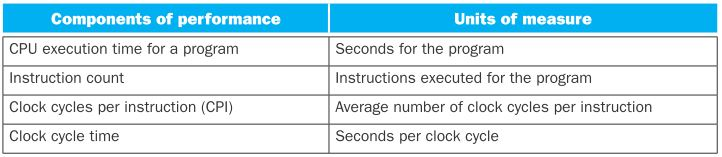
\includegraphics[scale=0.75]{Perform.JPG}
    \caption{Summary of basic components of performance}
\end{figure}

The performance of a program depends on:
\begin{itemize}
    \item The algorithm
    \item The language
    \item The compiler
    \item The architecture
    \item The actual hardware
\end{itemize}  

\begin{figure} [h!]
    \centering
    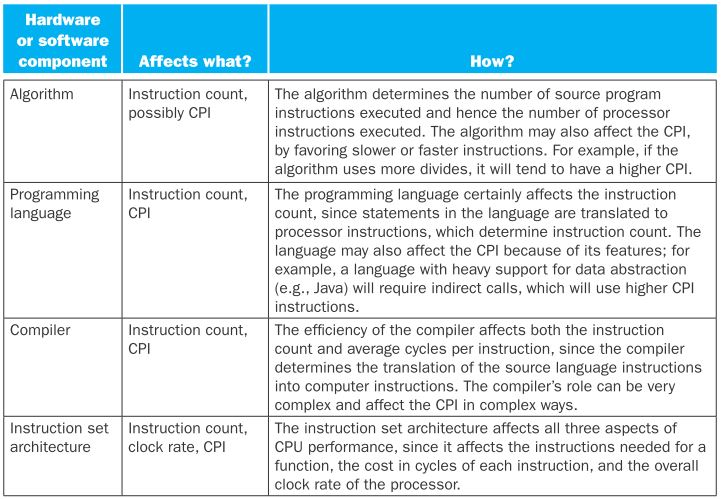
\includegraphics[scale=0.75]{Instruction.JPG}
\end{figure}

\pagebreak

%%%%%%%%%%%%%%%%%%%%%%%%%%%%%%%%%%%%%%%%%%%%%%%%%%%%%%%%%%%%%%%%%%%%%%%%%%%%%%%%%%%%%%%%%%%%%%%%%%%%%%%%%%
\section{Power wall}

\begin{figure} [h!]
    \centering
    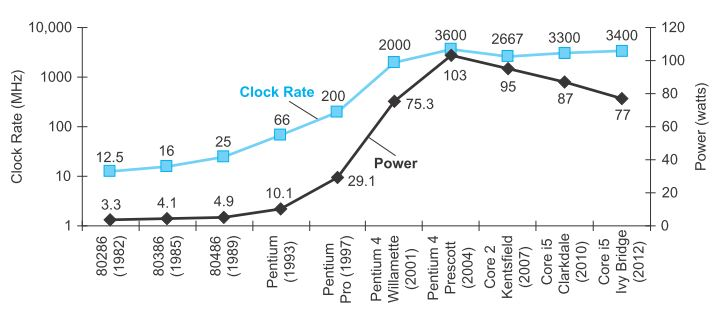
\includegraphics[scale=0.8]{CPU.JPG}
\end{figure}

Note both clock rate and power increased rapidly for decades, and then flattened off recently. The
reason for the growth together is that it is correlated, and the reason for the recent slowing is
due to the practical power limit for cooling commodity microprocessors.

Energy is a critical resource. Battery life is more important than performance in the personal
mobile device, and the architects of warehouse scale computers try to reduce the  costs of powering
and cooling $100 000$ servers as the costs are high at this scale. 

Just like measuring time in seconds is a safer measure of program performance than a 
rate like MIPS (see Section 1.10), the energy metric joules is a better measure than 
a power rate like watts, which is just joules/second.

The defining equation on CMOS integration technology is:
\begin{align*}
    \text{Power} = \text{Capacitative load}\times \text{Voltage}^2 \times \text{Frequency}
\end{align*}

\textbf{Example 1}: Given a new CPU that has 
\begin{itemize}
    \item $85\%$ the capacitative load of the old CPU
    \item Reduction of $15\%$ on the voltage and frequency
\end{itemize} 
\begin{figure} [h!]
    \centering
    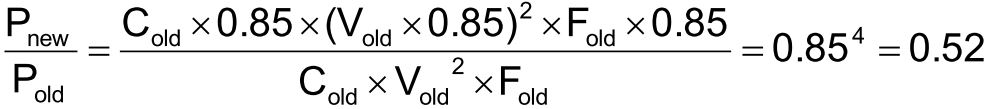
\includegraphics[scale=0.4]{Eq.JPG}
\end{figure}

\pagebreak

%%%%%%%%%%%%%%%%%%%%%%%%%%%%%%%%%%%%%%%%%%%%%%%%%%%%%%%%%%%%%%%%%%%%%%%%%%%%%%%%%%%%%%%%%%%%%%%%%%%%%%%%%%
\section{Uni-processors to multi-processors}

The power limit has forced a dramatic change in the design of microprocessors. Rather than
continuing to decrease the response time of a single program running on the single processor,
microprocessors, with multiple processors per chip, have the benefit of more on throughput rather
than on response time.s

In the past, programmers could rely on innovations in hardware, architecture, and compilers to
double performance of the programs. Today, for programmers to get significant improvement in program
response time, programs need to be written to take advantage of multiple processors. 

\textbf{Parallelism} has always been critical to performance in computing. A common example being
pipelining, an technique that runs programs faster by overlapping the execution of instructions.
This example is a form of instruction-level parallelism, where the parallel nature of the hardware
is abstracted  away so the programmer and compiler can think of the hardware as executing
instructions sequentially. 

Parallelism has always been less emphasised to programmers due to the following reasons:
\begin{itemize}
    \item Parallel programming is by definition performance programming, which increases the difficulty of programming.
    \item To be fast in parallel hardware, the programmer must divide an application so that each
    processor has roughly the same amount to do at the same time and that the overhead of scheduling
    and coordination reduce the potential performance benefits of parallelism. 
\end{itemize}

\pagebreak

%%%%%%%%%%%%%%%%%%%%%%%%%%%%%%%%%%%%%%%%%%%%%%%%%%%%%%%%%%%%%%%%%%%%%%%%%%%%%%%%%%%%%%%%%%%%%%%%%%%%%%%%%%
\section{Performance and ISAs}

ISAs have a big influence on performance, good and bad.
\begin{itemize}
    \item Good: ISAs may expose optimisation opportunities with compilers targeting specific
    instructions and ISA flexibility making it easier to tune micro-architecture.
    \item Bad: ISAs can act as a performance constraint by making it difficult to compile code efficiently
    and introduce complex critical path.
\end{itemize} 

As ISAs are meant to be stable and last for many years, it is a careful balancing act between:
\begin{itemize}
    \item Consistency and regularity for compilers
    \item Flexibility and opportunities for micro-architecture
\end{itemize}

There are two general approaches to ISAs:
\begin{figure} [h!]
    \centering
    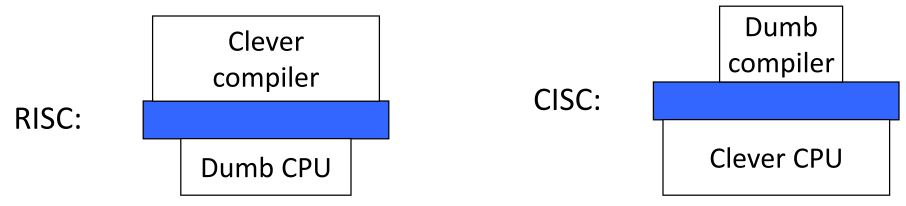
\includegraphics[scale=0.5]{ISA.JPG}
\end{figure}
\begin{itemize}
    \item CISC: 
    \begin{itemize}
        \item Dense code, simple compiler
        \item Powerful instruction set, variable format
    \end{itemize}
    \item RISC:
    \begin{itemize}
        \item Simple instructions, fixed format, optimising compiler
        \item Speed, low development cost, adapt to new technology
    \end{itemize}
\end{itemize}

\pagebreak

%%%%%%%%%%%%%%%%%%%%%%%%%%%%%%%%%%%%%%%%%%%%%%%%%%%%%%%%%%%%%%%%%%%%%%%%%%%%%%%%%%%%%%%%%%%%%%%%%%%%%%%%%%
\section{Memory}

\begin{figure} [h!]
    \centering
    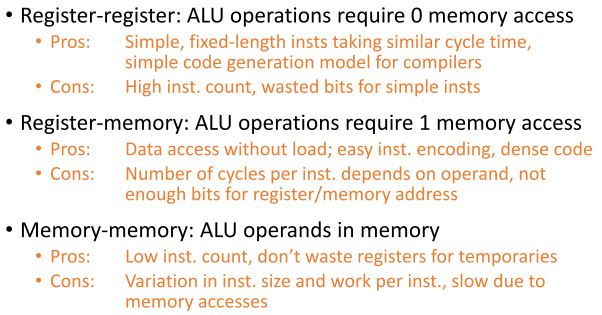
\includegraphics[scale=0.8]{Memo.JPG}
\end{figure}



\pagebreak

%%%%%%%%%%%%%%%%%%%%%%%%%%%%%%%%%%%%%%%%%%%%%%%%%%%%%%%%%%%%%%%%%%%%%%%%%%%%%%%%%%%%%%%%%%%%%%%%%%%%%%%%%%
\end{document}